\chapter{Introduction to Embedded Systems and Toolchain}

\section{The Chain of Evidence and the Bare-Metal Toolchain}
Building a bare-metal firmware relies on a strict \textbf{chain of evidence}. Every tool in the build pipeline has a specific, essential job to connect your C source code to the physical hardware. 

Here is exactly what each component does in practice:

\begin{itemize}
    \item \textbf{Cross-Compiler (e.g., \texttt{arm-none-eabi-gcc}):} Your PC cannot run microcontroller code. The cross-compiler's job is to translate your human-readable C code into the exact binary language that the target CPU understands (for the Cortex-M3, this is the \textbf{Thumb-2} instruction set).
    
    \item \textbf{Linker and Linker Script (\texttt{.ld}):} The compiler creates isolated blocks of code, but the CPU needs them placed at specific physical addresses. The linker glues these blocks together, using the \textbf{linker script} as a map. It dictates that executable code and constants must be saved in permanent \textbf{Flash} memory, while writable variables must be placed in volatile \textbf{SRAM}.
    
    \item \textbf{Hardware Vector Table:} A fixed directory located at the very beginning of the memory (address \texttt{0x00000000}). When powered on, the CPU is "blind" and reads the first two entries here to know how to start:
    \begin{enumerate}
        \item The first word tells the CPU where to place its temporary working memory (the \textbf{Main Stack Pointer}).
        \item The second word tells the CPU the exact address of the first instruction to execute (the \textbf{Reset Handler}).
    \end{enumerate}
    
    \item \textbf{Startup Code (Reset Handler):} A crucial piece of code that runs \textit{before} your \texttt{main()} function. Its job is to "prepare the house" (the RAM) for your application. It performs two critical tasks:
    \begin{enumerate}
        \item \textbf{Data Initialization:} It copies variables that have a starting value (e.g., \texttt{int x = 5;}, the \texttt{.data} section) from the permanent Flash into the working SRAM.
        \item \textbf{BSS Clearing:} It fills variables that have no starting value (the \texttt{.bss} section) with zeros directly in SRAM.
    \end{enumerate}
    Only after the RAM is perfectly set up, the startup code safely calls \texttt{main()}.
\end{itemize}

Understanding what each component actually does transforms debugging. If a program crashes before even reaching \texttt{main()}, a developer immediately knows to check the linker script or the startup code, rather than the application logic.

\section{What is an Embedded Operating System?}
An operating system (OS) manages hardware resources for applications. General-Purpose OS use a Memory Management Unit (MMU) to isolate applications in virtual memory. 

An \textbf{Embedded Operating System (EOS)} is completely different: it is a highly specialized, tightly constrained OS built to execute a single, fixed workload on a specific hardware device.

\subsection{Key Properties of Embedded Systems}
\begin{itemize}
    \item \textbf{Resource Constraints:} Built for kilobytes of RAM/Flash and milliwatts of power. Zero overhead allowed.
    \item \textbf{Real-Time Determinism (RTOS):} Deadlines matter as much as logic. A correct calculation delivered late (e.g., in an airbag sensor) is a total system failure. Predictability beats raw speed.
    \item \textbf{Flat Memory Architecture:} No virtual memory. The kernel, drivers, and tasks share one physical address space and are compiled into a single firmware image.
    \item \textbf{Static Configuration:} Since the workload is fixed at compile time, dynamic memory allocation (\texttt{malloc}) is rarely used. Tasks, memory pools, and hardware resources are statically allocated.
\end{itemize}

\begin{figure}[h]
    \centering
    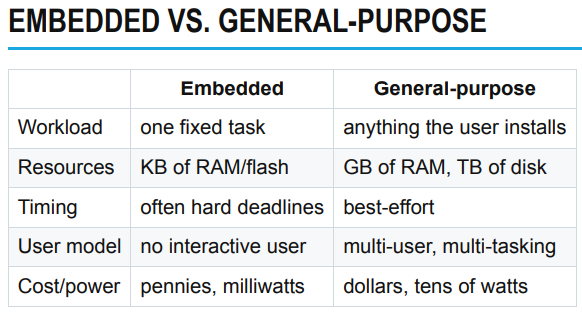
\includegraphics[width=0.4\textwidth]{contents/images/EvsGP.png}
    \caption{Embedded vs General Purpose OS characteristics.}
\end{figure}

\section{Operating System Architectures}

\subsection{Monolithic OS Structure}
The entire operating system runs as a single, large program in a privileged kernel space.
\begin{itemize}
    \item \textbf{Unified Kernel:} Core services (scheduling, memory, file systems, drivers) live together.
    \item \textbf{Maximum Throughput:} Components share the same memory and communicate directly without message-passing overhead.
    \item \textbf{The Risk:} If one driver crashes, the entire system halts (e.g., Linux, Windows).
\end{itemize}

\begin{figure}[h]
    \centering
    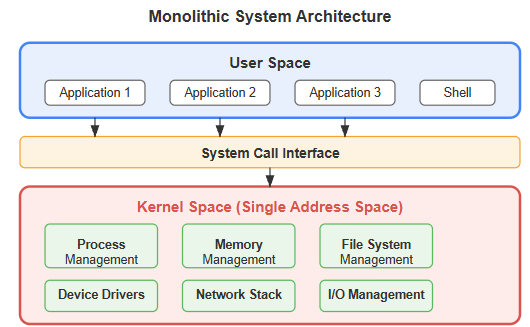
\includegraphics[width=0.3\textwidth]{contents/images/Monolithic.png}
    \caption{Monolithic Operating System Structure.}
\end{figure}

\subsection{Microkernel OS Structure}
A minimalist design that keeps only essential features (scheduling, basic memory management, IPC) in privileged mode. Everything else runs as isolated user-space apps.
\begin{itemize}
    \item \textbf{Fault Containment (Advantage):} High security and reliability. If a device driver crashes, it restarts independently without bringing down the core OS.
    \item \textbf{Performance Penalty (Disadvantage):} Slower than monolithic systems. Isolated components must constantly talk via Inter-Process Communication (IPC), causing heavy context-switching overhead.
\end{itemize}

\begin{figure}[h]
    \centering
    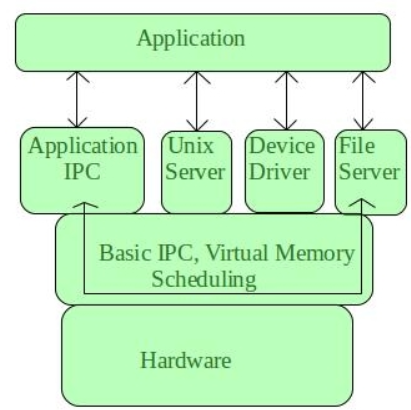
\includegraphics[width=0.3\textwidth]{contents/images/Microkernel.png}
    \caption{Microkernel Operating System Structure.}
\end{figure}

\subsection{Flat OS Structure (Bare-Metal)}
The simplest architecture, where there are no layers or isolated spaces.
\begin{itemize}
    \item \textbf{Single Linked Image:} The startup code, OS kernel, device drivers, and apps are merged into one executable stored in Flash. No dynamic app loader.
    \item \textbf{Raw Physical Memory:} Everything maps directly to raw physical addresses. No MMU translation.
    \item \textbf{No Hardware Isolation:} No protection boundaries between kernel and user space.
\end{itemize}

\textbf{Advantages:}
\begin{itemize}
    \item \textbf{High Speed:} Zero latency from OS abstractions or IPC.
    \item \textbf{Simplicity:} Easy to build and deploy for small, dedicated hardware.
\end{itemize}

\textbf{Disadvantages \& Risks:}
\begin{itemize}
    \item \textbf{Zero Isolation:} A single bug (e.g., a bad pointer) in any task can overwrite the entire system memory and cause a hard crash.
    \item \textbf{Blocking Tasks:} A stuck function or infinite loop halts the entire CPU.
    \item \textbf{Poor Scalability:} Unmanageable as code complexity grows.
\end{itemize}


\subsection{What we will do in the course?}
\textbf{The starting point (\textit{scratch-os}):} The course begins by building \textit{scratch-os}, which utilizes a \textbf{\textit{flat firmware architecture}}. This exposes the entire internal pipeline, from the initial boot process to task scheduling, making the hardware assumptions completely visible and non-negotiable.

\textbf{The transition (FreeRTOS):} Later, we transition to FreeRTOS, a production-ready RTOS closer to a microkernel philosophy. It features a small dedicated kernel and implements real scheduling policies (though, by default, it does not enforce memory protection). The educational goal is clear: \textbf{\textit{using a high-level RTOS API is easy only when you already understand the invisible state transitions happening underneath it}}.

The exact \textbf{\textcolor{red}{sequence of core mechanisms}} you will build manually:
\begin{enumerate}
    \item \textbf{Reset}: Handling the initial hardware state upon power-up.
    \item \textbf{Initialize memory}: Setting up the RAM (copying `.data`, zeroing `.bss`) so C code can safely execute.
    \item \textbf{Start application}: Transitioning control to the application logic.
    \item \textbf{React to events \& Schedule}: Handling hardware interrupts and deciding which task gets CPU time next.
    \item \textbf{Synchronize}: Ensuring tasks do not corrupt shared data or peripherals.
\end{enumerate}

\section{The Target Machine: Cortex-M3 and QEMU}
Embedded software is built for a known processor and a fixed memory map. It cannot rely on an OS to create a process, assign an address space, or arrange standard I/O. 

\subsection{Microcontroller (MCU) vs General-Purpose CPU}
A \textbf{microcontroller (MCU)} integrates onto a single chip the components that a desktop computer splits across a motherboard.
\begin{itemize}
    \item \textbf{Integration}: A desktop CPU is just a processing core requiring external buses for RAM and I/O. An MCU has the CPU, RAM, Flash, and Peripherals (Timers, UART, GPIO) built directly into the same chip.
    \item \textbf{Memory Management}: Desktop CPUs use an MMU to provide isolated virtual address spaces. An MCU relies on a \textbf{\textit{single flat physical address map}} shared by code, data, and peripherals (No MMU).
    \item \textbf{Hardware Interaction}: On an MCU, hardware is simply memory you write to directly. There is no abstraction layer between your code and a device register.
\end{itemize}

\subsection{The QEMU target (\texttt{mps2-an385})}
Instead of physical hardware, the course uses \textbf{QEMU}, a software emulator. Specifically, it targets the \texttt{mps2-an385} machine, which models an \textbf{ARM Cortex-M3} processor. The linker script strictly defines its physical memory map:
\begin{itemize}
    \item \textbf{FLASH (Origin: \texttt{0x00000000}, 4 MiB):} Non-volatile. Holds the initial image: vector table, executable instructions (`.text`), and read-only constants (`.rodata`).
    \item \textbf{SRAM (Origin: \texttt{0x20000000}, 4 MiB):} Volatile. Holds mutable state: initialized globals (`.data`), zero-initialized globals (`.bss`), the heap, and the stack. 
    \item \textbf{The Stack:} It starts at the very top of the RAM (\texttt{0x20400000}) and \textbf{\textit{grows downwards}} to lower addresses.
\end{itemize}

\subsection{Peripheral Registers and the \texttt{volatile} Keyword}
In later weeks, device drivers will interact with peripherals by reading/writing to fixed memory addresses. These memory accesses MUST be declared \textbf{\texttt{volatile}} in C. 
\begin{itemize}
    \item \textbf{Why \texttt{volatile}?}: It tells the compiler that the value at that memory address can change outside the program's control (e.g., a hardware sensor updating), or that a write triggers a physical effect. Without \texttt{volatile}, the compiler's optimizer might delete the memory access, assuming it's an unused ordinary variable. 
    \item \textit{Note:} \texttt{volatile} does \textbf{not} provide atomicity or concurrency protection; it only ensures the access is physically executed by the CPU.
\end{itemize}







\section{Technical Foundations \& Toolchain}

\subsection{From Source Code to a Running Program}
The goal of this phase is to understand how to compile and run an application step by step, working directly with commands without relying on an IDE (like Visual Studio Code). Often, development environments hide the real compilation process behind a simple "Play" button, but when developing operating systems, it is essential to understand what actually happens under the hood.

The toolchain is a pipeline composed of several small tools, where the output of one becomes the input of the next:
\begin{itemize}
    \item \textbf{C Preprocessor:} manages and expands directives like \texttt{\#include} and \texttt{\#define}.
    \item \textbf{Compiler:} takes the preprocessed code and generates assembly code (\texttt{.s}).
    \item \textbf{Assembler:} converts the assembly into machine code, producing object files (\texttt{.o}).
    \item \textbf{Linker:} concatenates matching sections, resolves symbols to final addresses, and through an \texttt{.ld} script, generates the final binary image (the ELF image).
\end{itemize}

% \includegraphics[width=0.8\textwidth]{images/toolchain_pipeline.png}
% Suggested caption: Toolchain pipeline from C source to ELF image

\subsection{Why Cross-Compilation?}
Developing for embedded systems introduces an architectural problem: the computer we are writing the code on (Host) is different from the machine where the code will be executed (Target)[cite: 1]. The host is typically an x86-64 or Apple Silicon machine, whereas our target is an ARM Cortex-M3 processor[cite: 1].

A normal \texttt{gcc} compiler installed on the computer emits code optimized for the machine it runs on, which makes it useless for our purpose[cite: 1]. For example, a recent Mac's native compiler would generate code for a 64-bit ARM architecture, while our target board requires code for a 32-bit ARM architecture.

For this reason, a \textbf{cross-compilation toolchain} (specifically \texttt{arm-none-eabi-*}) is required[cite: 1]. It runs on the host but generates code for the target's ISA (Instruction Set Architecture)[cite: 1].

The \texttt{none-eabi} nomenclature is crucial to understand the environment we are working in:
\begin{itemize}
    \item \textbf{none:} indicates the absence of a host operating system on the target (bare-metal development)[cite: 1].
    \item \textbf{eabi:} indicates the use of the standard embedded ARM ABI (Application Binary Interface)[cite: 1].
\end{itemize}

Working in a "bare-metal" environment means not having the standard libraries typical of desktop operating systems: there will be no \texttt{printf} to a console, no \texttt{malloc} dynamic allocation supported by an OS, and no \texttt{\_start} function from a C library unless we explicitly provide it[cite: 1].

\subsubsection{Checking the Toolchain: Host vs Target}
To concretely verify the difference between compilers, we can simply query the toolchain from the terminal:
\begin{itemize}
    \item By running \texttt{gcc -dumpmachine}, you get the architecture of your host machine (e.g., a 64-bit architecture for a recent desktop system)[cite: 1].
    \item By running \texttt{arm-none-eabi-gcc -dumpmachine}, the output will clearly indicate a 32-bit ARM architecture followed by the \texttt{none} environment.
\end{itemize}

Getting two completely different target strings for the same command typed on the same computer demonstrates the fundamental concept of a cross toolchain[cite: 1]. When writing an operating system from scratch, it is imperative to use this type of compiler, generate the binary file, transfer it to the target machine, and finally run it.


\subsection{Host, Target, and Emulator}
During the development of software for embedded systems, it is essential to keep three key roles distinct in the compilation and testing process[cite: 1]:
\begin{itemize}
    \item \textbf{Host:} This is the PC we work on (e.g., our laptop) and where the text editor, toolchain, and other development tools are executed[cite: 1].
    \item \textbf{Target:} This is the physical hardware destination machine (in our case, a board with an ARM Cortex-M3 processor) for which the executable (the ELF image) is generated[cite: 1].
    \item \textbf{Emulator:} This is a virtual machine that simulates the target's hardware via software directly on our host[cite: 1]. In our case, lacking the physical board, we will use \textbf{QEMU} to test the execution of the programs[cite: 1].
\end{itemize}

\subsection{Reset Code and the Transition to C}
When running a program on a desktop computer, the operating system and the C runtime take care of preparing the memory and starting the program automatically[cite: 10]. In a bare-metal environment, at boot time, no such service exists[cite: 10]. 

To execute even just the first instruction of our \texttt{main()} function, it is necessary to have startup code (\texttt{boot/startup.c}) that acts as the bridge between the reset hardware and the application[cite: 10]. 

This code is responsible for making the C runtime's assumptions true before \texttt{main()} runs: it guarantees that every global variable already has its promised value (by initializing the \texttt{.data} and \texttt{.bss} memory sections) by the time \texttt{main()} starts[cite: 10].

The startup source also defines crucial bare-metal safety mechanisms:
\begin{itemize}
    \item \textbf{\texttt{Default\_Handler}:} An infinite loop used for unimplemented exception vectors. Stopping in that known loop is much safer and more diagnosable than falling into arbitrary memory after an unexpected hardware exception.
\end{itemize}

\subsection{Preprocessing: Assemble the Translation Unit}
When we start compiling (e.g., by typing the classic \texttt{gcc} command), the process is not monolithic but is divided into very distinct phases. The very first phase is handled by the \textbf{C preprocessor}. 
The preprocessor analyzes the C source code looking for directives (commands starting with the \texttt{\#} character, such as \texttt{\#include} or \texttt{\#define}) and expands these macros before the compiler actually sees the program[cite: 1]. 

This is purely text substitution, without any machine code generation[cite: 1]. For example, upon encountering an \texttt{\#include} command, the preprocessor locates the specified file and essentially "copies and pastes" it into the source file, replacing the original directive.
The result of this operation is a \textit{translation unit}: a single file of pure C code with all macros and headers already expanded[cite: 1].

\subsubsection{Try It: Preprocess Only}
We can instruct the toolchain to run \textit{only} the preprocessing phase by using the \texttt{-E} flag. The command to run in the terminal is the following[cite: 1]:

\texttt{arm-none-eabi-gcc -mthumb -mcpu=cortex-m3 -nostartfiles -ffreestanding -E src/main.c -o build/main.i}

In this string, we provide several options to describe to the toolchain the characteristics of the machine we actually have available[cite: 1]:
\begin{itemize}
    \item \texttt{-mthumb} and \texttt{-mcpu=cortex-m3}: these indicate, respectively, to use the Thumb instruction set and that the target CPU is a Cortex-M3[cite: 1].
    \item \texttt{-nostartfiles} and \texttt{-ffreestanding}: these signal that we are working in a bare-metal environment, meaning without standard operating system libraries or default startup files[cite: 1]. These options will be the default for our projects.
    \item \texttt{-E}: commands the compiler to stop immediately after preprocessing[cite: 1].
\end{itemize}

If we open the generated output file (\texttt{main.i}), we will notice fundamental changes compared to the original source:
\begin{enumerate}
    \item All text comments present in the source have been removed by the preprocessor.
    \item The \texttt{\#include <stdint.h>} directive has disappeared, entirely replaced by the expanded text (the typedef definitions) contained in that header file[cite: 1].
    \item The original C code of the \texttt{main()} function has remained textually identical at the bottom of the file[cite: 1].
\end{enumerate}
This demonstrates that the actual compiler, in subsequent steps, will never read our original \texttt{main.c}, but will work on this "translated" file (\texttt{main.i}), which can become huge if there are many files to include.

\subsection{Compilation: C Becomes Target Instructions}
Once preprocessing is finished, the compiler itself comes into play. The role of this step is to check the C syntax and translate the preprocessed code into \textbf{assembly} code specific to our target architecture[cite: 1]. 
All the options we provided earlier (such as \texttt{-mcpu}) are needed precisely by the compiler to know exactly which instructions to generate for 32-bit ARM microprocessors.

\subsubsection{Compilation and Target Architecture}
There are many 32-bit ARM microprocessors available, so it is necessary to specify the exact model being used, which in our case is the Cortex-M3. This specific CPU supports the Thumb instruction set (Thumb-2)[cite: 1]. Therefore, the compiler must be instructed precisely about the target CPU by providing specific options[cite: 1]. Finding the correct configuration involves matching the hardware datasheet specifications with the extensive GCC compiler documentation. Once the correct configuration is established and understood, it can be seamlessly applied to all future projects running on that same target machine.

\subsubsection{Try It: Stop After Compilation}
To observe the compilation phase without proceeding further in the pipeline, we can run the compiler using the \texttt{-S} flag (instead of the \texttt{-E} flag used for preprocessing)[cite: 1]. The \texttt{-S} option instructs the toolchain to run the preprocessor, compile the code, and stop immediately after producing the assembly version of the C program[cite: 1].
    
The output is typically stored in a file with a \texttt{.s} extension, such as \texttt{main.s}. Opening this file reveals that the original high-level C program has been translated into low-level ARM assembly instructions[cite: 1]. These instructions are written using human-readable mnemonics, not raw binary code, proving that the compiler's role at this specific stage is purely translation into assembly language[cite: 1]. While reading these files is not strictly required for this course, it is crucial to know that this intermediate translation step always takes place.

\subsection{Assembly: Instructions Become Relocatable Bytes}
Once the assembly version of the code is generated, the next tool in the chain is the \textbf{Assembler}. Its role is similar to a compiler, but it specifically takes the assembly code (\texttt{.s}) and translates it into binary machine code[cite: 1]. 

The output of this phase is an \textbf{object file} (identifiable by the \texttt{.o} extension). However, it is important to emphasize that the binary code contained in an object file is still not executable firmware[cite: 1]. Because projects are usually composed of multiple source files, the assembler processes each file in complete isolation. As a result, the generated object files contain machine-code bytes, section names, and symbol definitions, but they still lack proper, final memory addresses[cite: 1]. They may also contain unresolved references to code located in other object files (for instance, \texttt{startup.o} referring to \texttt{main}), which cannot be resolved at this stage[cite: 1].

\subsubsection{Try It: Assemble to an Object File}
To run the complete compiling chain up to the end of the assembly phase (executing preprocessing, compiling, and assembling sequentially), the \texttt{-c} flag must be used[cite: 1]. We can apply this to the different source files in our project:
\begin{itemize}
    \item \texttt{arm-none-eabi-gcc [...] -c boot/startup.c -o build/boot/startup.o}[cite: 1]
    \item \texttt{arm-none-eabi-gcc [...] -c src/main.c -o build/src/main.o}[cite: 1]
\end{itemize}

By doing this, we generate the object files \texttt{startup.o} and \texttt{main.o}. Unlike the previous \texttt{.i} and \texttt{.s} files, these object files represent the first output in the pipeline that is entirely in binary format[cite: 1]. Opening them with a standard text editor will reveal unreadable characters, as they are no longer in a human-readable format.


\subsubsection{Inspecting Object Files}
To understand what is inside an object file, we can use a tool provided by our toolchain called \texttt{arm-none-eabi-nm}[cite: 1]. This tool reads the \texttt{.o} files and extracts information in a human-readable way, specifically focusing on "symbols"[cite: 1]. 

Symbols represent the memory addresses that our program uses, which at this assembly stage are still left open and undefined[cite: 1]. For example, if we run the tool on our object files, we can look for the \texttt{main} function:
\begin{itemize}
    \item In \texttt{startup.o}, there is a call to the \texttt{main} function, but it is not defined there. The tool will label this symbol with a \textbf{U} (Undefined), meaning it is referenced but its address is unknown[cite: 1].
    \item In \texttt{main.o}, the function is actually written and defined. The tool will label this symbol with a \textbf{T} (indicating it is defined in the \texttt{.text} section)[cite: 1].
\end{itemize}
This separation is completely normal: the files are compiled in isolation, and it will be the linker's job to connect the "U" to the "T" and assign the final memory addresses[cite: 1].

\subsection{Linking: Creating the Executable}
As established, object files are not runnable firmware[cite: 1]. In ARM architecture, every assembly line corresponds to a 32-bit instruction with a fixed binary encoding. However, whenever an instruction needs to reference a memory address (like calling a function), those bits are left blank and filled with symbols instead. 

To convert these isolated objects into a final executable, we need a last step: the \textbf{Linker}[cite: 1]. The linker takes all the independent object files, concatenates matching sections, resolves every symbol to a final address, and patches all the references[cite: 1]. The output is an executable file formatted as \textbf{ELF} (Executable and Linking Format), which is the standard format originally designed in Unix and used globally (unlike the proprietary \texttt{.exe} format used by Windows)[cite: 1].

\subsubsection{The Linker Script}
When compiling a program on a standard PC, the operating system manages memory automatically, so the linker already knows what to do[cite: 1]. However, in a bare-metal embedded system, there is no operating system to rely on[cite: 1]. 

Therefore, we must explicitly instruct the linker on how to organize the different pieces of code in memory using a \textbf{Linker Script} (usually a \texttt{.ld} file)[cite: 1]. This script specifies the physical addresses of the hardware, detailing exactly what goes into the Flash memory (e.g., \texttt{.text}, \texttt{.rodata}) and what goes into the SRAM (e.g., \texttt{.data}, \texttt{.bss}, stack)[cite: 1]. Without this script, the toolchain wouldn't know the chip's specific memory map[cite: 1].

\subsubsection{Try It: Link the Objects}
If we want to run the compiler without stopping at intermediate steps and link the project, the command becomes more complex because we must include the linker script and all the necessary object files[cite: 1]. 

The command looks like this:
\texttt{arm-none-eabi-gcc [...] -T scripts/mps2\_m3.ld [...] build/boot/startup.o build/src/main.o -o build/scratch-os.axf}[cite: 1]

Here, the \texttt{-T} flag is crucial because it tells the compiler which linker script to use (\texttt{scripts/mps2\_m3.ld})[cite: 1]. After running this, we obtain our final, linked ELF image (\texttt{scratch-os.axf}). If we inspect it again with \texttt{arm-none-eabi-nm}, the \texttt{main} symbol will no longer be marked as "U" (undefined), but will have a finalized memory address assigned by the linker[cite: 1].


\subsubsection{The Linker Script and the Map File}
To perform the final link, the linker needs a strict description of physical memory[cite: 14]. To provide this, the link command in the Makefile uses specific flags assigned to the \texttt{LDFLAGS} variable:

\begin{lstlisting}[language=make]
LDFLAGS := -T scripts/mps2_m3.ld
LDFLAGS += -Xlinker -Map=build/output.map
\end{lstlisting}

\begin{itemize}
    \item \textbf{The Linker Script (\texttt{-T}):} The first option chooses the course linker script (\texttt{scripts/mps2\_m3.ld})[cite: 14]. The script begins by declaring the \texttt{FLASH} and \texttt{RAM} regions, then specifies the output sections that occupy them. Its internal syntax defines how it places the vector table so the processor finds it at reset, how it splits an initialized global's storage between a Flash load address and a RAM run address, and how it reserves the heap and stack. While writing this script from scratch is a Week 2 topic, for now, it is provided as-is to make the build work.
    
    \item \textbf{The Map File (\texttt{-Map}):} The second option emits a map file (\texttt{build/output.map})[cite: 14]. This file is an invaluable explanation of exactly where the linker placed each input contribution and symbol[cite: 14]. 
\end{itemize}

For Week 1, reading the generated map file is enough evidence that the script successfully assigned the final addresses and generated a valid executable binary file[cite: 14].

\subsection{The ELF Image and its Map}
The final target file generated by the toolchain is \texttt{build/scratch-os.axf}. The \texttt{.axf} suffix is commonly used for an ARM executable containing debug information, but the underlying file format is standard \textbf{ELF (Executable and Linkable Format)}[cite: 14, 15]. 

The ELF file organizes the program into several useful views[cite: 15, 16]:
\begin{itemize}
    \item \textbf{Sections:} Serve the linker and debugger (e.g., \texttt{.text}, \texttt{.rodata}, \texttt{.data}, \texttt{.bss})[cite: 15, 16].
    \item \textbf{Program Headers:} Describe memory ranges that a loader (or QEMU) places in memory[cite: 15].
    \item \textbf{Symbols:} Assign human-readable names to final physical addresses.
\end{itemize}

\subsubsection{Thumb State and The Entry Point}
The Week 1 build generates a 32-bit, little-endian ARM ELF executable. Running the command \texttt{arm-none-eabi-readelf -h -S build/scratch-os.axf} extracts the ELF header and reports the entry point at \texttt{0x49}[cite: 15]. 

However, looking at the map file, the \texttt{Reset\_Handler} is located at \texttt{0x00000048}. This mismatch is not an error: the low bit in the ELF entry address (\texttt{0x49} vs \texttt{0x48}) explicitly records the \textbf{Thumb state}. They describe the exact same execution entry, but the \texttt{+1} tells the CPU to execute in Thumb-2 mode.

\subsubsection{Sections Layout in Week 1}
The generated ELF contains the following allocated sections mapping directly to the physical addresses dictated by the linker script:

\begin{lstlisting}
.isr_vector  address 0x00000000  size 0x40
.text        address 0x00000040  size 0xa0
.data        address 0x20000000  size 0x0
.bss         address 0x20000000  size 0x0
.heap        address 0x20000000  size 0x1000
\end{lstlisting}

The map file (\texttt{build/output.map}) explicitly tracks this derivation[cite: 14]. It records the 64-byte vector table at Flash address zero, followed by the startup code (\texttt{startup.o}) at \texttt{0x40}. The application code (\texttt{main.o}) begins at \texttt{0xa4}, and the \texttt{"toolchain OK\char`\\n"} string literal is placed in \texttt{.rodata} at \texttt{0xd0}. 

\subsubsection{File Size vs RAM Usage}
In this specific Week 1 snapshot, the \texttt{.data} and \texttt{.bss} sections have a size of \texttt{0x0}. This should \textbf{not} be misread as evidence that RAM initialization is optional in bare-metal systems[cite: 10, 16]. It merely indicates that this specific, tiny program has no global variables needing those regions yet[cite: 16].

To accurately verify memory usage, developers run \texttt{arm-none-eabi-size build/scratch-os.axf}[cite: 17]. For Week 1, it reports 224 bytes of text, 0 bytes of data, and 4096 bytes of \texttt{bss}[cite: 17]. Note that this 4096-byte \texttt{bss} total includes the \texttt{.heap} section, deliberately reserved in the linker layout to occupy RAM[cite: 17].
\subsection{Debug Information for Host Tools}
When an operating system is finalized and released, information about the original source code is typically stripped from the binary to reduce size and protect intellectual property. However, during development and debugging, it is highly beneficial to generate binary files that contain debugging information[cite: 48]. 

Specific compiler options can embed source-level debug metadata inside the ELF[cite: 48]. This does not mean the target machine understands C; it still only runs machine instructions[cite: 48]. Instead, this metadata allows host-side tools (like QEMU or a debugger) to associate a specific binary instruction address with a corresponding C file line, function, or variable[cite: 48]. This bridge between high-level C code and low-level execution makes investigating crashes possible without altering the basic boot image[cite: 48].

\subsection{What Make Actually Does}
While it is crucial to understand how to compile an embedded program manually, step by step, doing so in practice is extremely inefficient[cite: 49]. Remembering every compiler flag, every linker script option, and listing every single C file becomes impossible for complex projects (for instance, the FreeRTOS kernel consists of hundreds of C files)[cite: 49]. 

To automate the compilation process, we use tools like \textbf{Make}, which is the standard toolchain automation used by Linux and FreeRTOS[cite: 49]. A \texttt{Makefile} is essentially a text-based script that defines a set of rules to compile many files[cite: 49]. 

\subsubsection{Targets Model Desired Outcomes}
The \texttt{Makefile} works by defining \textbf{targets} and the actions required for each target[cite: 50]. A target is a named file or action that Make knows how to produce[cite: 50]. For example, if you have a target named \texttt{all}, you can simply type \texttt{make all} in the terminal, and the tool will execute all the instructions associated with that target[cite: 50]. Some targets, like \texttt{clean} or \texttt{run}, are usually actions rather than actual files, and they are declared as \texttt{.PHONY} to prevent conflicts with a same-named file[cite: 50].

Make is also powerful because it tracks \textbf{prerequisites} (the dependency graph)[cite: 50, 54]. If you specify that the linking step requires all object files to be created first, Make will search for the rule to generate those object files if they do not exist[cite: 50, 54]. It works backward, starting from the desired result and executing all the necessary preceding steps[cite: 50, 54].

\subsubsection{Prerequisites Capture Rebuild Logic}
Another key feature of Make is its ability to rebuild a target only if a prerequisite is newer than the target itself[cite: 49, 51]. For example, if you change one variable in a massive project (like the Linux kernel, which can take hours to compile), you do not want to recompile everything[cite: 49, 51]. Make identifies that only one \texttt{.c} file has changed, recompiles that specific file into an object file, and then simply re-runs the linker to update the final ELF image[cite: 49, 51].

To identify if something has changed, Make uses the last modified timestamp of the files[cite: 51]. However, this can sometimes lead to issues. If you are using version control (like Git) or syncing folders via cloud services (like OneDrive or Dropbox), file timestamps can become corrupted or mistakenly set in the future. In these cases, you might modify a file, but Make will refuse to recompile it because it believes the target is already up-to-date. If you encounter strange build behaviors, checking the timestamps of your files is an excellent troubleshooting step.

\subsection{Variables and Compiler Flags}
The Makefile uses a simple language that allows the definition of variables. Variables are incredibly useful because they centralize configuration: you define them once and use them throughout the script.

For instance, the compiler flags encode crucial information such as the target architecture, warning policies, optimization levels, include paths, and bare-metal assumptions. The Makefile's core flags make the target policy explicit:

\begin{lstlisting}[language=make]
CFLAGS := -mthumb -mcpu=cortex-m3 -nostartfiles -std=gnu17
CFLAGS += -Wall -Wextra -O0 -g3
\end{lstlisting}

These are not just personal preferences, but a strict contract for the build:
\begin{itemize}
    \item \texttt{CC}: Chooses the cross-compiler (e.g., \texttt{arm-none-eabi-gcc}). The "none" nomenclature explicitly means "No OS," which has practical consequences: there is no host-supplied \texttt{\_start}, no dynamic loader, no process to return to when \texttt{main()} finishes, and no guaranteed \texttt{printf} console.
    \item \texttt{-mthumb -mcpu=cortex-m3}: Selects the exact instruction subset implemented by the target.
    \item \textbf{\texttt{-nostartfiles}}: This is particularly important. It prevents the toolchain's usual C startup objects from taking responsibility for the reset. It forces the system to rely on our custom \texttt{boot/startup.c} to make that responsibility visible.
    \item \texttt{-O0 -g3}: Disables optimizations (\texttt{-O0}) and includes maximum debug symbols (\texttt{-g3}). This favors a debuggable, source-corresponding image over an optimized one.
    \item \texttt{LDFLAGS}: Governs memory layout and the final link.
\end{itemize}

\subsubsection{Build Directories Keep Artifacts Separate}
In a well-structured \texttt{Makefile}, it is common practice to save the generated executable file and intermediate objects in a dedicated directory, often named \texttt{build}[cite: 53]. 

Using a build directory provides several benefits[cite: 53]:
\begin{itemize}
    \item Source directories remain readable and uncluttered[cite: 53].
    \item The \texttt{clean} target can remove generated files safely without risking the deletion of source code[cite: 53].
    \item Different configurations can coexist in separate build folders[cite: 53].
    \item A fresh build tests whether the dependencies are complete[cite: 53].
\end{itemize}
It is crucial to remember never to manually edit the generated object files or ELF bytes in the build directory in an attempt to change program behavior[cite: 53]. All changes must originate from the source code.

\subsubsection{Variables and String Manipulation in Make}
Using variables in a \texttt{Makefile} is not strictly mandatory; you could write raw commands by skipping variables entirely if your script consists of just one command[cite: 52]. However, it is a highly recommended practice for clean and maintainable code. By saving compiling information (such as the compiler name, the target executable name, or the \texttt{build} directory path) into variables, you create a single point of entry[cite: 52, 53]. If, for instance, you decide to switch to another compiler, you only need to change one line, and the rest of the file will still function perfectly[cite: 52]. Variables in Make are essentially strings, and you can perform both variable assignment and variable concatenation[cite: 52].

Make also possesses a powerful language for processing strings and performing replacements, somewhat similar to regular expressions. This is particularly useful when managing source files. 
Instead of manually writing the compiling command for 100 different C files, you can list all the \texttt{.c} files in a \texttt{SOURCES} variable[cite: 54]. Then, you can use a short string substitution command to automatically generate the list of object files (\texttt{OBJECTS})[cite: 54]. For example, the command can parse the \texttt{SOURCES} string, split it by slashes to remove the original directory (e.g., \texttt{boot} or \texttt{src}), prepend the \texttt{build} directory, and replace the \texttt{.c} extension with \texttt{.o}[cite: 54]. This automation is why Make is an indispensable tool in large projects[cite: 54].

\subsection{Defining Targets and Rules}
The fundamental unit Make reasons about is the \textbf{rule}. A Makefile is composed of targets (what you want to execute) and the exact instructions to execute them[cite: 18]. 

The syntax for a rule involves a target on the left of a colon, followed by its dependencies (prerequisites), and then the recipe:
\begin{lstlisting}[language=make]
target: prerequisite1 prerequisite2
    recipe line 1
    recipe line 2
\end{lstlisting}

\begin{itemize}
    \item \textbf{Target:} Normally a file Make knows how to produce (e.g., an object file or ELF image), or an action (like \texttt{clean} or \texttt{run})[cite: 16, 18]. Actions must be explicitly declared as \texttt{.PHONY} to prevent Make from looking for a file with that name[cite: 16, 18].
    \item \textbf{Prerequisites:} Files that must already be current before the recipe runs. Make's rebuild decision compares modification times: a target is out of date (and its recipe runs) if it does not exist, or if any prerequisite's timestamp is newer than the target's[cite: 16].
    \item \textbf{Recipe:} The sequence of shell commands that turns the prerequisites into the target. 
\end{itemize}

\textbf{\textcolor{red}{Crucial Syntax Rule:}} Every recipe line \textbf{MUST} start with a literal \texttt{Tab} character, not spaces. This is the single most common syntax error in a first Makefile.

\subsubsection{Diagnosing the "Missing Separator" Error}
If you indent a recipe line with four spaces instead of a Tab, Make will crash and report a cryptic error like:
\begin{lstlisting}[language=bash]
Makefile:5: *** missing separator.  Stop.
\end{lstlisting}
The "separator" Make refers to is the Tab character it required to recognize line 5 as a recipe. Finding spaces instead, it tried to parse the line as a variable assignment or a new rule, and failed. 

Because four spaces and a Tab look identical in an editor, do not inspect the line by simply reading it. Render its whitespace in the terminal using \texttt{cat -et Makefile}. This command marks the end of each line with \texttt{\$} and each Tab with \texttt{\textasciicircum I}, making the missing Tab immediately obvious. To avoid this entirely, configure your editor to never expand Tabs to spaces in Makefiles.

\subsubsection{Variable Assignment Types and Debugging}
Make variables centralize configuration, but how you assign them matters[cite: 17, 18]:
\begin{itemize}
    \item \texttt{:=} (Simply expanded): The right-hand side is evaluated once, immediately. This is the preferred method.
    \item \texttt{=} (Recursively expanded): The right-hand side is re-evaluated every time the variable is used. This can be slow or cause infinite loops.
    \item \texttt{+=}: Appends to whatever the variable already holds.
\end{itemize}

By convention, uppercase names like \texttt{CC}, \texttt{CFLAGS}, and \texttt{LDFLAGS} are reserved for tools and flags, while lowercase names are for internal bookkeeping[cite: 17, 18].

\textbf{Making a Makefile Report its Own State:}
A Makefile can be wrong without failing (e.g., if a substitution is subtly incorrect). To debug what variables actually expanded to, you can ask the Makefile directly using \texttt{\$(info ...)} or \texttt{\$(warning ...)}:
\begin{lstlisting}[language=make]
$(info OBJECTS = $(OBJECTS))
$(warning CFLAGS is $(CFLAGS))
\end{lstlisting}
These directives are expanded while the Makefile is being \textit{read}, not built, and they print their values to the console regardless of the target you are building, making them excellent temporary debugging aids.

\subsubsection{Automatic Variables}
Inside a recipe, a handful of special variables refer back to the rule that triggered it, so the same pattern rule can serve every matching file without repeating filenames[cite: 18]:
\begin{itemize}
    \item \textbf{\texttt{\$@}}: The target of this rule[cite: 18].
    \item \textbf{\texttt{\$<}}: The first prerequisite[cite: 18].
    \item \textbf{\texttt{\$\^}}: All prerequisites, space-separated, duplicates removed[cite: 18].
    \item \textbf{\texttt{\$(dir \$@)}}: The directory part of \texttt{\$@} (a built-in function)[cite: 18].
\end{itemize}

The Week 1 pattern rule uses exactly these to automatically create build directories and compile every source file[cite: 18]:
\begin{lstlisting}[language=make]
$(BUILD_DIR)/%.o: %.c
	@mkdir -p $(dir $@)
	$(CC) $(CFLAGS) -c $< -o $@
\end{lstlisting}

\subsubsection{Pattern Rules and Substitution References}
A \textbf{pattern rule} (\texttt{\%.o: \%.c}) uses a stem \texttt{\%} that matches on both sides of the colon. Given a request to build an object file, Make matches it automatically without needing one explicit rule per file[cite: 19]. 

Additionally, a \textbf{substitution reference} like \texttt{\detokenize{\$(SOURCES:\%.c=\$(BUILD_DIR)/\%.o)}} acts as a shorthand to convert the source list into the corresponding object file list.

\subsubsection{Phony Targets}
Actions like \texttt{run} and \texttt{clean} do not name actual files that Make should create[cite: 19]. Using \textbf{\texttt{.PHONY}} tells Make that a target is not a file, ensuring its recipe always runs when requested and preventing conflicts if a file with the same name exists[cite: 19]. \texttt{all} is the conventional default goal[cite: 19].

\subsubsection{Reading the Week 1 Makefile as a Dependency Graph}
Put together, the checkpoint's complete \texttt{Makefile} is structured as a dependency graph[cite: 20]:

\begin{lstlisting}[language=make]
SOURCES := boot/startup.c src/main.c
OBJECTS := $(SOURCES:%.c=$(BUILD_DIR)/%.o)

.PHONY: all clean run
all: $(BIN)

$(BUILD_DIR)/%.o: %.c
	@mkdir -p $(dir $@)
	$(CC) $(CFLAGS) -c $< -o $@

$(BIN): $(OBJECTS)
	$(CC) $(CFLAGS) $(LDFLAGS) $(OBJECTS) -o $(BIN)

run: $(BIN)
	qemu-system-arm ...

clean:
	rm -rf $(BUILD_DIR)
\end{lstlisting}

Running \texttt{make} walks this graph bottom-up[cite: 20]. This provides the core reproducibility benefit: the graph records how the image is made, and re-running it is always correct whether nothing changed, one file changed, or the build directory does not exist yet[cite: 20].

\subsubsection{A Disciplined First Build Loop}
The \texttt{Makefile} operates on a dependency graph[cite: 54]. For instance, if the target executable (\texttt{\$(BIN)}) cannot be generated because the object files (\texttt{.o}) are missing, Make searches for the rule that dictates how to create them[cite: 54]. 

This rule typically looks like this:
\texttt{\$(BUILD\_DIR)/\%.o: \%.c}[cite: 54]

This means that for every \texttt{.o} file on the left side, the dependency is the corresponding \texttt{.c} file on the right side[cite: 54]. If the \texttt{.o} file is missing or outdated, this rule is triggered[cite: 54]. The actions associated with this rule usually involve:
\begin{enumerate}
    \item Creating the \texttt{build} folder if it does not already exist.
    \item Running the compiler with the \texttt{-c} flag, which instructs it to compile and stop before linking[cite: 54].
\end{enumerate}

When you simply type \texttt{make}, the tool executes these rules in reverse order: it checks for the final ELF file, realizes it needs the object files, realizes it needs to compile the source files, and then executes the steps sequentially from the bottom up. 
This provides a highly disciplined build loop: you can run \texttt{make} to build the ELF, inspect the terminal for any compiler errors, run the generated ELF, and compare the observed output with what you expect[cite: 55].

\subsection{QEMU Runs a Board Model}
The final crucial target in our \texttt{Makefile} is the \texttt{run} command[cite: 54]. 
The rule for \texttt{run} depends on \texttt{\$(BIN)}: the finalized ELF file must be available before execution can begin[cite: 54]. If the file is present, Make executes QEMU (\texttt{qemu-system-arm})[cite: 56].

The emulator requires several parameters to function correctly:
\begin{itemize}
    \item \texttt{-machine mps2-an385}: This tells QEMU which specific hardware board it needs to emulate, ensuring the CPU and memory map match our Cortex-M3 target[cite: 56].
    \item \texttt{-kernel}: This parameter passes the generated ELF file to the emulator[cite: 56].
\end{itemize}
Other options might include disabling the graphical screen (since we only need the terminal output) and enabling semi-hosting to emulate a debugging cable attached to the board. 

When this command runs, QEMU emulates the entire physical process: it acts as if a program has flashed the ELF into memory, the power is turned on, and the board starts executing[cite: 56].

\subsection{QEMU, Semihosting, and the Observed Result}
The \texttt{run} target first ensures the ELF exists, then invokes QEMU with specific parameters: \texttt{-machine mps2-an385}, \texttt{-kernel build/scratch-os.axf}, \texttt{-nographic}, and semihosting enabled. QEMU supplies the target-side machine model while presenting its console directly through the host terminal.

\subsubsection{Why Avoid \texttt{printf}?}
The application in \texttt{src/main.c} intentionally avoids standard \texttt{printf}. The custom reset path does not perform the complete C-library initialization expected by newlib's semihosting-backed stdio. 

Instead, \texttt{semihost\_write0} makes the ABI-level request directly:
\begin{enumerate}
    \item Places semihosting operation \texttt{0x04} (\texttt{SYS\_WRITE0}) in register \texttt{r0}.
    \item Places the NUL-terminated message pointer in register \texttt{r1}.
    \item Executes the Thumb breakpoint instruction \texttt{bkpt 0xab}.
\end{enumerate}
With semihosting enabled, QEMU intercepts the breakpoint trap, writes the requested string to the host console, and resumes target execution.

\subsubsection{Running the Demonstration}
To execute the demonstration from the checkpoint directory:
\begin{lstlisting}[language=bash]
make
make run
\end{lstlisting}

The observable terminal output is:
\begin{lstlisting}
toolchain OK
\end{lstlisting}

\subsubsection{Interpreting the Output}
After printing, \texttt{main()} returns to the \texttt{Reset\_Handler}, which enters its final infinite spin loop[cite: 21]. QEMU continues running because the target continues executing that loop; it must be interrupted manually[cite: 21]. 

Therefore, the single line \texttt{toolchain OK} is \textbf{not} an exit notification. It is concrete, empirical evidence that the image successfully reached the intended point in the boot path[cite: 21].

\subsubsection{The Final Spin Loop and QEMU Execution}
It is important to note what happens after the \texttt{main()} function finishes its execution. \texttt{main()} itself never returns to an operating system because, in a bare-metal environment, there is no OS to return to[cite: 21]. 

When it does return, the \texttt{Reset\_Handler} enters a final \texttt{for( ;; ) \{\}} spin loop, because a bare-metal image has nowhere else to go[cite: 21]. This ensures the processor remains safely locked in a known state instead of wandering into uninitialized memory and executing random garbage data[cite: 21].

\textbf{Crucial Note on Emulator Behavior:} QEMU keeps running that infinite loop; it does not exit on its own. Any explanation saying that QEMU automatically exits after printing the final message is strictly incorrect for this checkpoint.

\section{A Practical Inspection Routine}
When working on this checkpoint, it is essential to inspect the source and generated evidence in the exact order of the pipeline:
\begin{enumerate}
    \item \textbf{Read the \texttt{Makefile}} to see the commands and target flags.
    \item \textbf{Read the linker script (\texttt{mps2\_m3.ld})} to establish legal memory regions and section order.
    \item \textbf{Read \texttt{startup.c}} to see how linker symbols become initialization loops and how reset reaches C.
    \item \textbf{Read \texttt{main.c}} to identify the expected observable behavior.
    \item \textbf{Use map and ELF tools} to verify that the linker implemented the intended layout:
\end{enumerate}

\begin{lstlisting}[language=bash]
arm-none-eabi-readelf -h -S build/scratch-os.axf
arm-none-eabi-size build/scratch-os.axf
\end{lstlisting}

\subsection{Systematic Troubleshooting}
When faults occur during development, follow a systematic troubleshooting path:
\begin{itemize}
    \item \textbf{If the compiler rejects a command:} Check the cross-toolchain installation and the Makefile flags.
    \item \textbf{If a symbol is unresolved:} Check the object list and matching declarations.
    \item \textbf{If a section overflows:} Inspect the linker-script memory regions and the map file.
    \item \textbf{If QEMU starts but the expected output is absent:} Check the reset path, the call to \texttt{semihost\_write0}, and the semihosting options.
\end{itemize}

\subsection{Foundational Significance}
This checkpoint serves as the permanent foundation for all subsequent work: future peripherals will use the same physical-address model, task code will still enter through the same reset path, and every future image will be linked, inspected, and booted through this exact toolchain. Week 1 makes these relationships explicit before later operating system abstractions obscure them.